\documentclass[crop,tikz]{standalone}

\usepackage{amsmath,amssymb}

\begin{document}
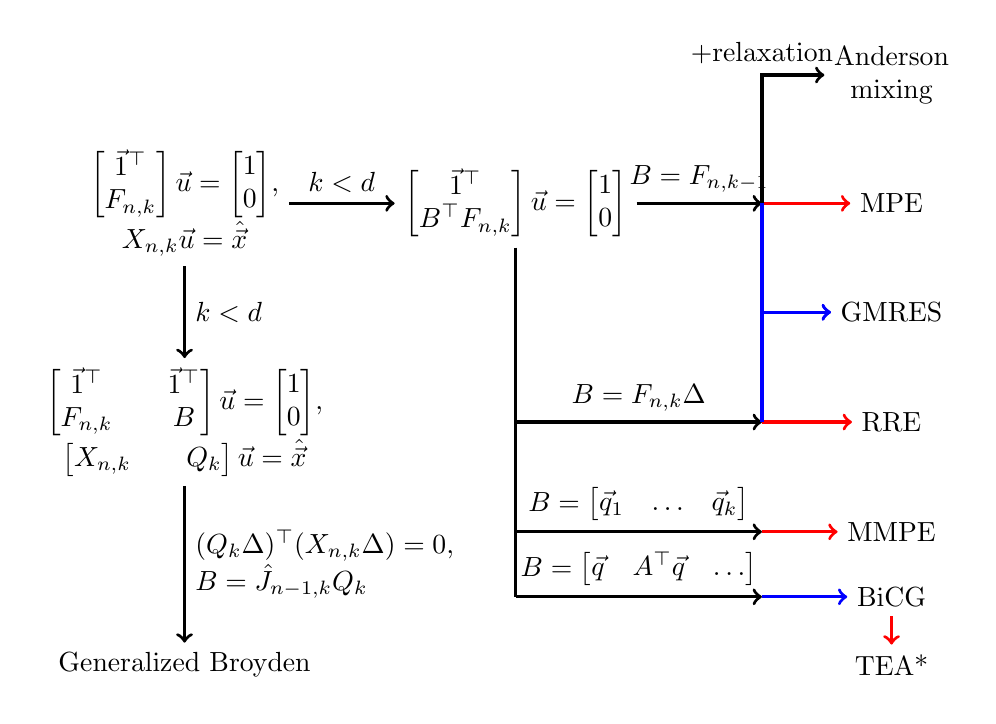
\begin{tikzpicture}
    \matrix (m) [column sep=0.8cm, row sep=1em, ampersand replacement=\&]{
      \& \& \& \& \node[align=center] (Anderson) {Anderson\\mixing}; \\
      \node[align=center] (multisecant) {$\begin{bmatrix} \vec{1}^\top \\ F_{n,k} \end{bmatrix} \vec{u} = \begin{bmatrix} 1 \\ 0 \end{bmatrix}$,\\ $X_{n,k} \vec{u} = \hat{\vec{x}}$}; \&
      \node (overdetermined) {$\begin{bmatrix} \vec{1}^\top \\ B^\top F_{n,k} \end{bmatrix} \vec{u} = \begin{bmatrix} 1 \\ 0 \end{bmatrix}$}; \& \&
      \node[coordinate] (preMPE) {}; \& \node (MPE) {MPE}; \\
      \& \& \& \& \node (GMRES) {GMRES}; \\
      \node[align=center] (preBroyden) {$\begin{bmatrix} \vec{1}^\top \& \vec{1}^\top \\ F_{n,k} \& B \end{bmatrix} \vec{u} = \begin{bmatrix} 1 \\ 0 \end{bmatrix}$,\\ $\begin{bmatrix} X_{n,k} \& Q_k \end{bmatrix} \vec{u} = \hat{\vec{x}}$};
      \& \node[coordinate] (prepreRRE) {}; \& \& \node[coordinate] (preRRE) {}; \& \node (RRE) {RRE}; \\
      \& \node[coordinate] (prepreMMPE) {}; \& \& \node[coordinate] (preMMPE) {}; \& \node (MMPE) {MMPE}; \\
      \& \node[coordinate] (preTEA) {}; \& \& \node[coordinate] (preBiCG) {}; \& \node (BiCG) {BiCG}; \\
      \node (Broyden) {Generalized Broyden};
      \& \& \& \& \node (TEA) {TEA*}; \\
      };
    \path[->,very thick]
      (multisecant) edge node[above] {$k < d$} (overdetermined) edge node[right] {$k < d$} (preBroyden)
      (preBroyden) edge node[right,align=left] {$(Q_k \Delta)^\top (X_{n,k} \Delta) = 0$, \\ $B = \hat{J}_{n-1,k} Q_k$} (Broyden)
      (overdetermined) edge node[above] {$B=F_{n,k-1}$} (preMPE)
      (preMPE) edge[red] (MPE)
      (prepreRRE) edge node[above] {$B=F_{n,k} \Delta$} (preRRE)
      (preRRE) edge[red] (RRE)
      (prepreMMPE) edge node[above] {$B=\begin{bmatrix} \vec{q}_1 & \dots & \vec{q}_k \end{bmatrix}$} (preMMPE)
      (preMMPE) edge[red] (MMPE)
      (preTEA) edge node[above] {$B=\begin{bmatrix} \vec{q} & A^\top \vec{q} & \dots \end{bmatrix}$} (preBiCG)
      (preBiCG) edge[blue] (BiCG)
      (BiCG) edge[red] (TEA);
    \draw[-, very thick] (overdetermined) edge (preTEA);
    \draw[->,very thick,blue] (preMPE) |- (GMRES);
    \draw[->,very thick,blue] (preRRE) |- (GMRES);
    \draw[->,very thick] (preMPE) |- node[above] {+relaxation} (Anderson);
  \end{tikzpicture}
\end{document}